\chapter{Introduction}

Hardware components are extremely complex. The main reasons for the
complexity is concurrency and the sheer size of components. For
examples, realistic processors make use of instruction pipelining to
execute multiple instructions concurrently. Complexity comes with such
concurrent executions, since one must ensure that they are executed
correctly. Size of components also grows by complexity. More realistic
processors require additional hardware components such as a reorder
buffer. The logic gets complicated again with these components.

Modularity has been considered as an effective way to design and
understand such complex hardware components. A complex hardware
component can can be constructed by composing several simple
modules. The notion of modules is so ingrained in that all commercial
Hardware Description Languages (HDLs) like Verilog, VHDL, Bluespec,
and Chisel~\cite{verilog, vhdl, bsdef, chisel} support the notion of
modules.

Among various HDLs, \Bluespec{}~\cite{bsdef, bsref} allows designers
to develop hardware not only based on modularity, but also based on
the notion of Guarded Atomic Actions (GAAs)~\cite{daniel-gaa}. Even
though most HDLs allow to design hardware in a modular manner, modules
cannot be independently designed if they are entangled with
clock-timing issues. For instance, when two modules, a producer of a
value and a consumer of that value, are connected with wires and the
producer is optimized to use fewer clock cycles to produce the value,
then the consumer should also be modified to consume the values
faster; failure to do so will result in an incorrect overall design.

Following the concepts of modularity and GAA, we have been defining a
framework called \Kami{}~\cite{kami-web, murali-thesis}, which is for
specifying, verifying, and synthesizing \Bluespec{}-style hardware
components. \Kami{} presents a domain specific language similar to
Bluespec. In addition, we define the formal semantics of the \Kami{}
language to enable proving properties of hardware. The framework has
been built on the Coq proof assistant; hence verification can be
performed by mechanized proofs with a high degree of automation.

The notion of modularity used in designing hardware can be extended to
verification. For modular verification, we want to be able to verify
the individual modules of a large system and compose their proofs to
verify the full system. In many cases, we reuse such simple components
in different larger designs. From the perspective of proof, reusing a
hardware component implies that we can also reuse its related
proofs. Thanks to the modular semantics in \Kami{}, it is indeed
possible to use the proof of a component whenever it is used in a
larger design.

Modules communicate with other modules by calling each other's
methods. In our modular semantics, we model these communications using
\emph{labels}. The semantics of these communicating modules is similar
to those of Labeled Transition Systems (LTS)~\cite{lts}. Each module
changes its internal state and potentially calls methods of other
modules during its state transition. These method calls become labels
in our semantics.  The modular semantics, therefore, also defines
behaviors of \emph{open systems}. Open systems have external
interactions, whose specifics cannot be figured out unless it is
connected with other modules which can respond to them.

However, modular semantics has an inherent weakness in that it is hard
to infer internal changes. Even if modular semantics allow us to
verify individual modules, we eventually should be able to understand
a part of design, which is still composed of several modules, when the
part cannot be decomposed anymore. In this case, modular semantics
defines behaviors of such modules by giving the behaviors of each
small modules \emph{for all possible combinations}. However, we
certainly do not want to consider such all cases, since we know only a
few cases are feasible by the design itself.

\begin{figure}[t]
  \centering
  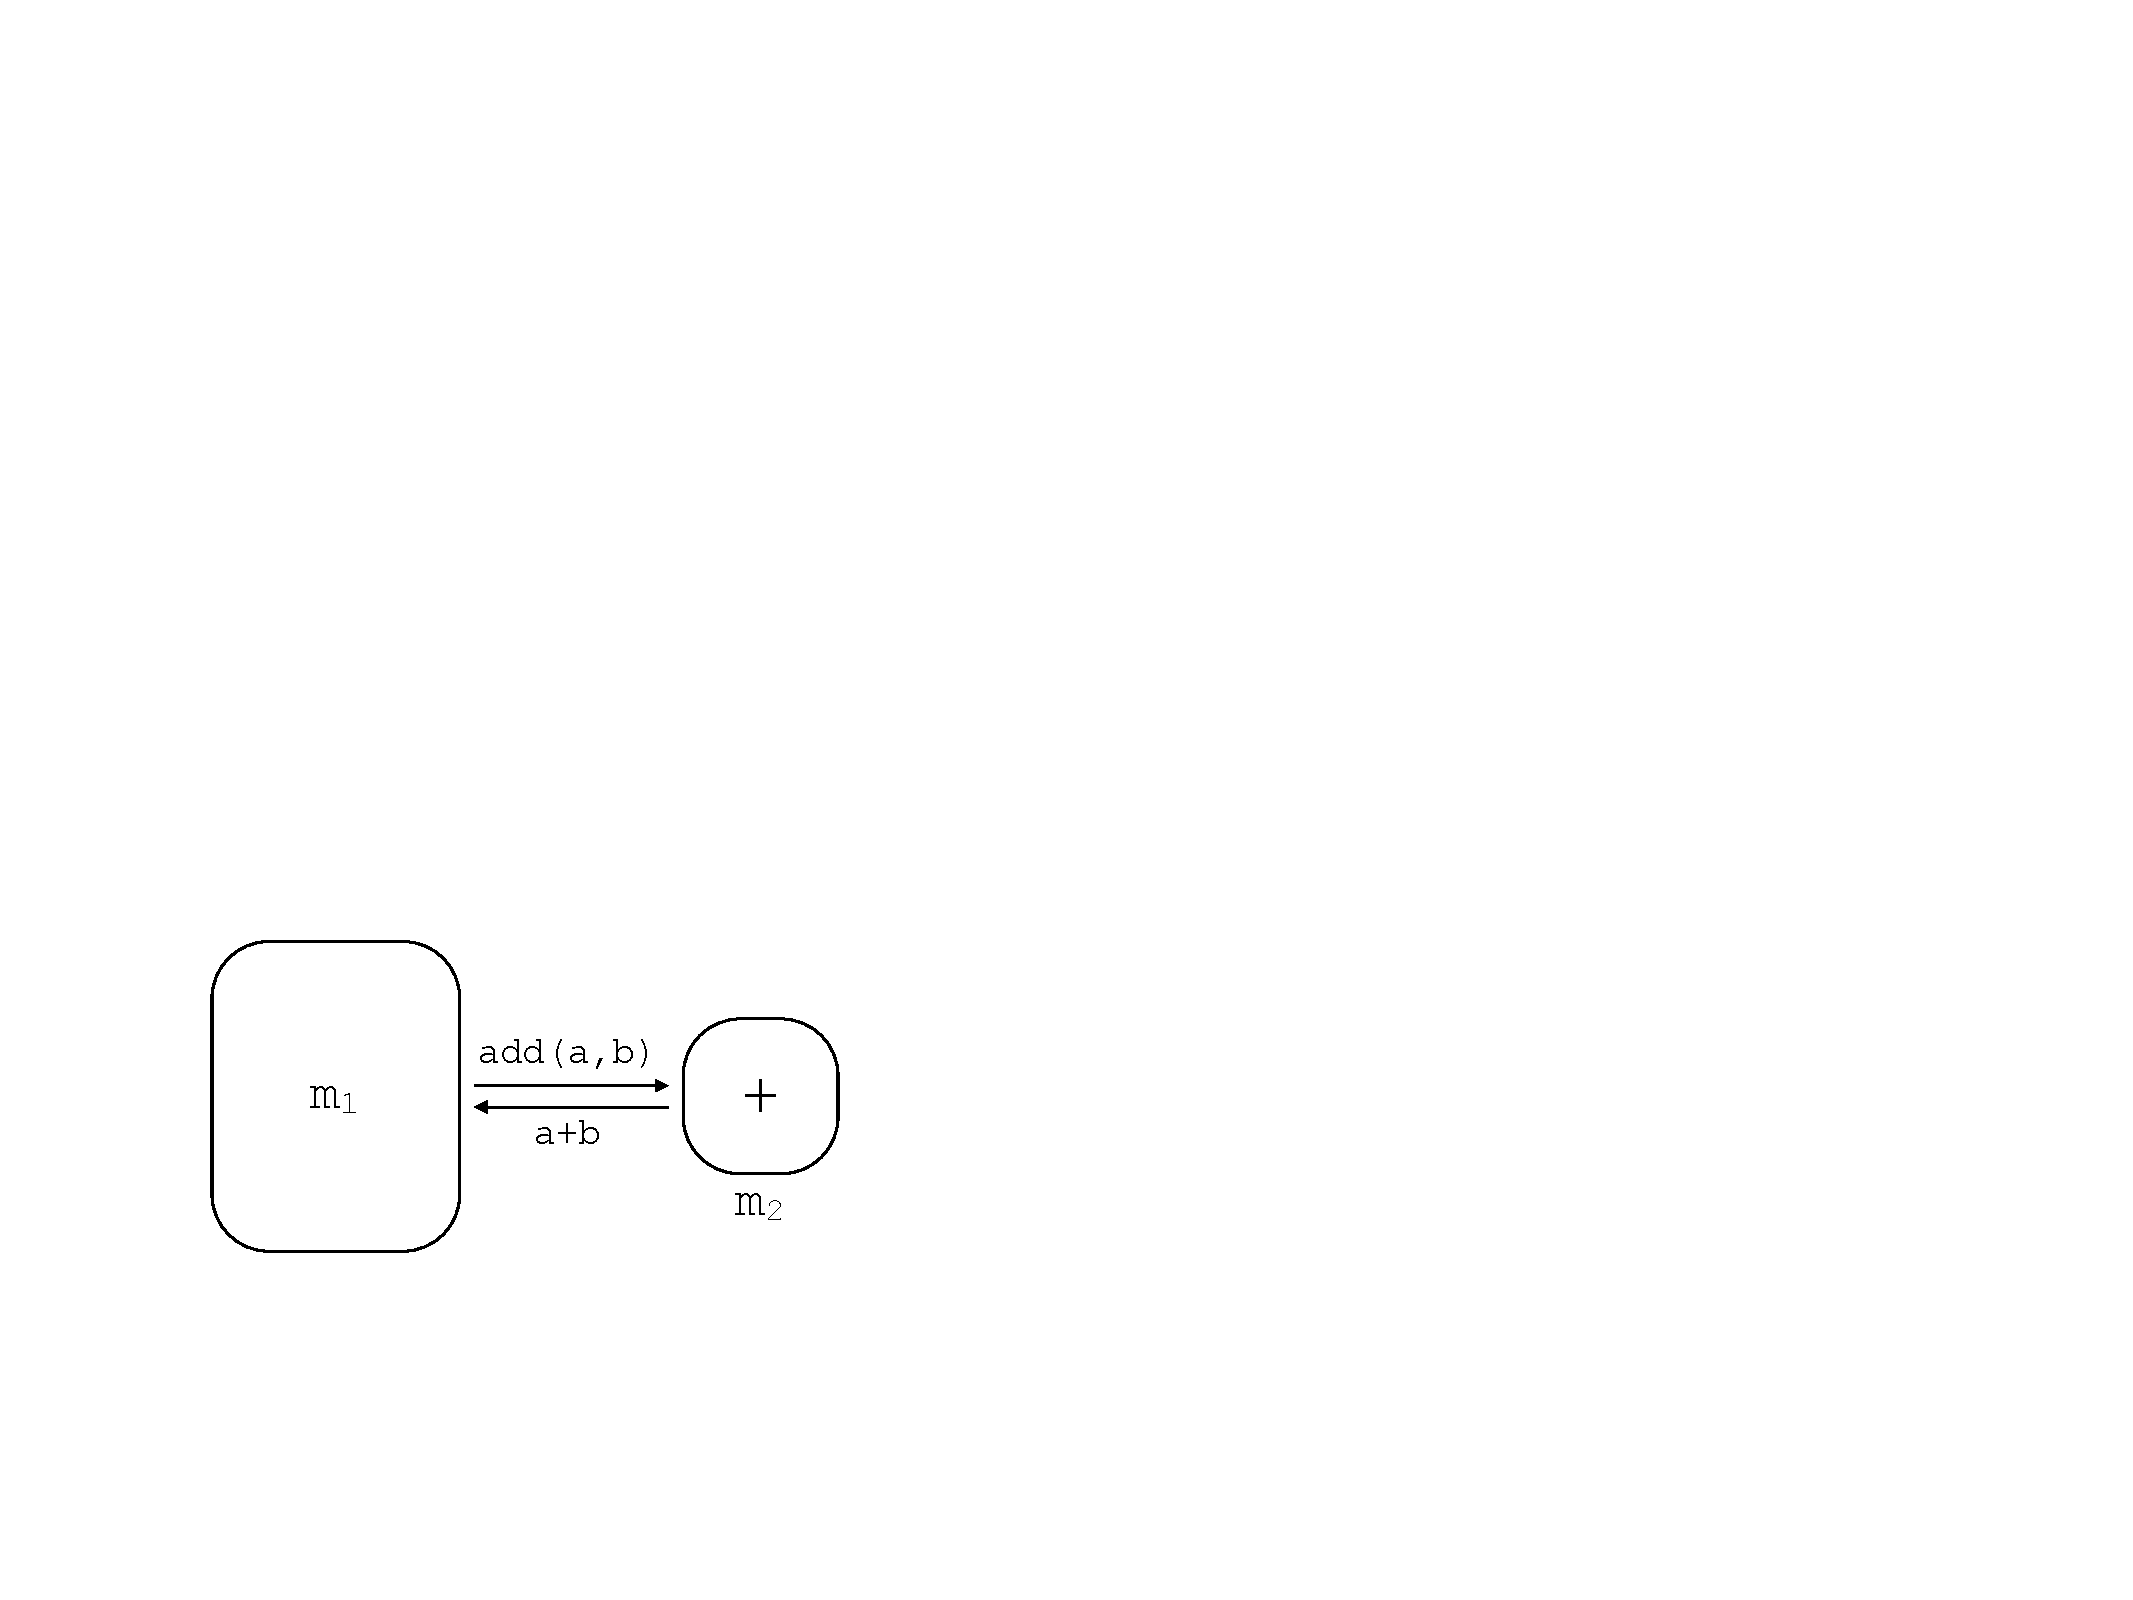
\includegraphics[width=0.5\textwidth]{figures/modsem-weakness.pdf}
  \caption{A weakness of the modular semantics}
  \label{ex-modular-semantics-weakness}
\end{figure}

A need for a new semantic approach rises more in terms of
verification. The semantics of a composition of two modules can be
understood by simply substituting the bodies of the methods in the two
modules at their respective places of calls,
like\ $\beta$-substitution.  The modular semantics, however, does not
perform such a syntactic substitution operation. Instead, it composes
the effects of the body of the method at its call site. This
definition poses a big problem in our verification effort. For
example, as shown in \reffig{ex-modular-semantics-weakness}, suppose
we have a module $m_1$ which calls the $\texttt{add}$ method of module
$m_2$ with two arguments and performs a state transition based on the
result. The semantics of the composed module $m_1 + m_2$ is defined
using the semantics of the body of the $\texttt{add}$ method and the
semantics of the state transition in $m_1$. Any analysis of the
composed module requires analyzing these two effects separately and
finally combining the effects. However, it is much simpler to analyze
the \emph{inlined} version of $m_1 + m_2$, where the body of method
$\texttt{add}$ is substituted into the body of the state transition of
$m_1$.

Hence, in this thesis, I present a new semantic approach, which is
based on inlining. Inlining semantics is defined for open hardware
systems and resolve the weakness by construction. The semantics uses a
static inlining operation to substitute internal calls to their method
bodies. This operator erases all internal calls in a module, so that
we do not need to care about internal communications.

An implication from the modular semantics to the inlining semantics is
also formally proven, thus it can be used in order to efficiently
prove properties of hardware. Since the two semantics does not have
equal capabilities, we give the implication proof saying that the
modular semantics imply the inlining semantics.

To sum up, the main contributions of this thesis are:
\begin{itemize}
\item To define a new semantic approach based on inlining, for open
  hardware systems.
\item To prove the implication from the modular semantics to the
  inlining semantics.
\end{itemize}

\paragraph{Overview}

The thesis is organized as follows: \refchap{chap:backgrounds}
introduces a number of prerequisites to understand the hardware design
concept of \Bluespec{}. Related works are also provided to compare
previous approaches to define hardware semantics.
\refchap{chap:semantics} presents the two semantics used in the
\Kami{} framework: modular and inlining
semantics. \refchap{chap:implication} compares capability of each
semantics and presents the implication proof between them. Lastly, we
draw conclusions and give future works in \refchap{chap:conclusions}.

